%%%mark = star, diamond, square, otimes
%\documentclass{article}
%\usepackage{pgfplots}
%\usepackage[justification=centering]{caption}
%\pgfplotsset{compat=newest}
%\begin{document}
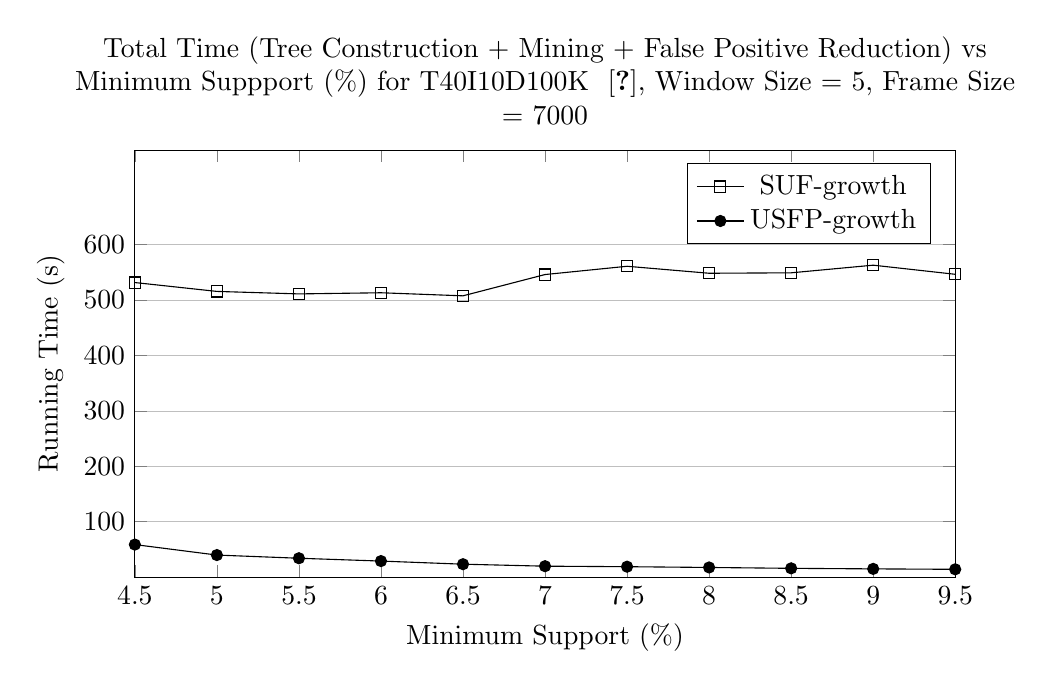
\begin{tikzpicture}
\begin{axis}[
	title={\parbox{\linewidth}{\centering  Total Time (Tree Construction + Mining + False Positive Reduction) vs Minimum Suppport (\%) for T40I10D100K ~\cite{dataset}, Window Size = 5, Frame Size = 7000}},
	width=12cm,
	height=7cm,
    xlabel={Minimum Support (\%) },
    ylabel={Running Time (s)},
    xmin=4.5, xmax=9.5,
    ymin=0, ymax=770,
    xtick={4.5,5,5.5,6,6.5,7,7.5,8,8.5,9,9.5},
    ytick={100,200,300,400,500,600},
    legend pos=north east,
    ymajorgrids=true,
    grid style={line width=.2pt,draw=gray!50},
]
 
\addplot[
    solid, every mark/.append style={solid, fill=gray}, mark=square
    ]
    coordinates {
			(4.5,531.579)
			(5  ,515.581)
			(5.5,511.075)
			(6  ,513.146)
			(6.5,507.618)
			(7  ,546.032)
			(7.5,560.952)
			(8  ,548.354)
			(8.5,549.139)
			(9  ,562.928)
			(9.5,546.47 )

};
    \addlegendentry{SUF-growth}
\addplot[
    solid, every mark/.append style={solid, fill=black}, mark=*
    ]
    coordinates {
			(4.5,58.652)
			(5  ,39.735)
			(5.5,33.993)
			(6  ,28.892)
			(6.5,23.262)
			(7  ,19.669)
			(7.5,18.735)
			(8  ,17.355)
			(8.5,15.785)
			(9  ,14.803)
			(9.5,14.013)

};
    \addlegendentry{USFP-growth}
 
\end{axis}
\end{tikzpicture}
%\end{document}